\section*{Задание 1. Сжатие изображений с помощью SVD}

В качестве исходного изображения использована картинка из набора по предмету, переведённая в оттенки серого и представлена в виде матрицы интенсивностей \(A\in\mathbb{R}^{m\times n}\).

Было выполнено SVD-разложение \(A = U\,\Sigma\,V^\top\), после чего построены укороченные аппроксимации \(A_k = U_{[:,1:k]}\,\Sigma_{1:k,1:k}\,V_{[1:k,:]}\) для ряда значений \(k\). Ниже приведены исходное изображение и сетка реконструкций для девяти значений \(k\), а также графики ошибки восстановления (MSE) и относительного объёма хранения.

\begin{figure}[h!]
  \centering
  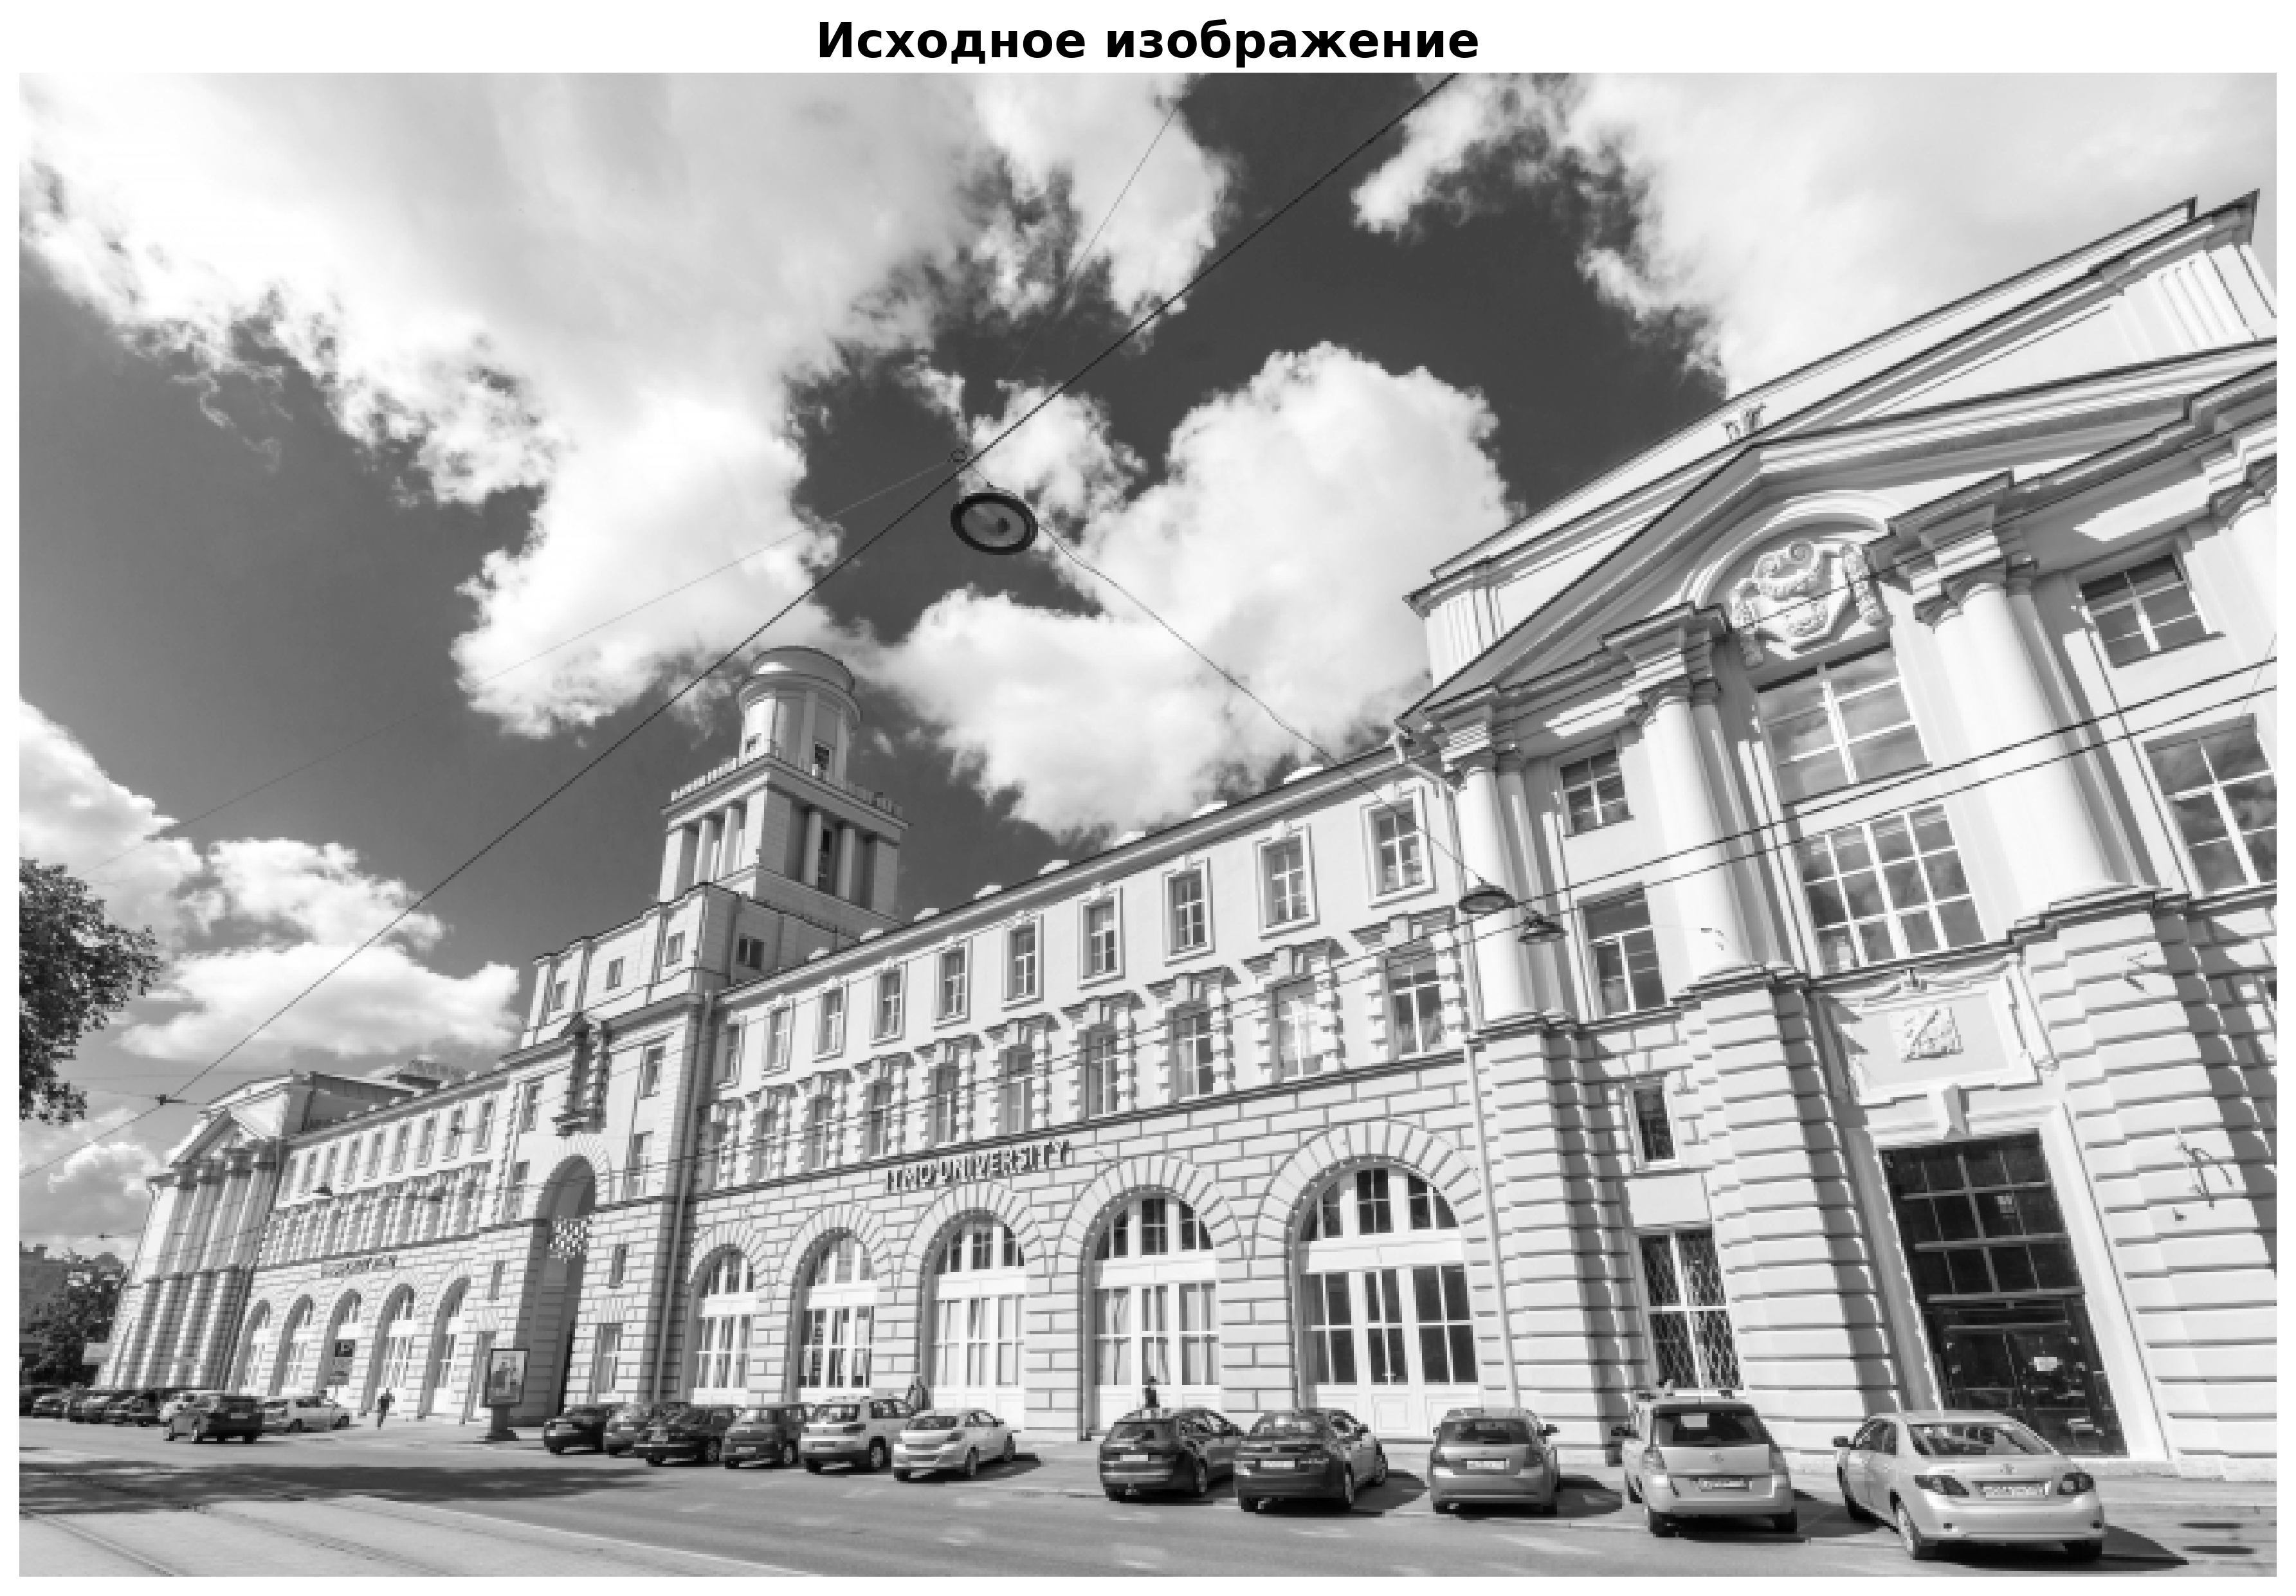
\includegraphics[width=0.6\linewidth]{images/task1/svd_original.png}
  \caption{Исходное изображение в оттенках серого}
  \label{fig:svd-original}
\end{figure}

\begin{figure}[h!]
  \centering
  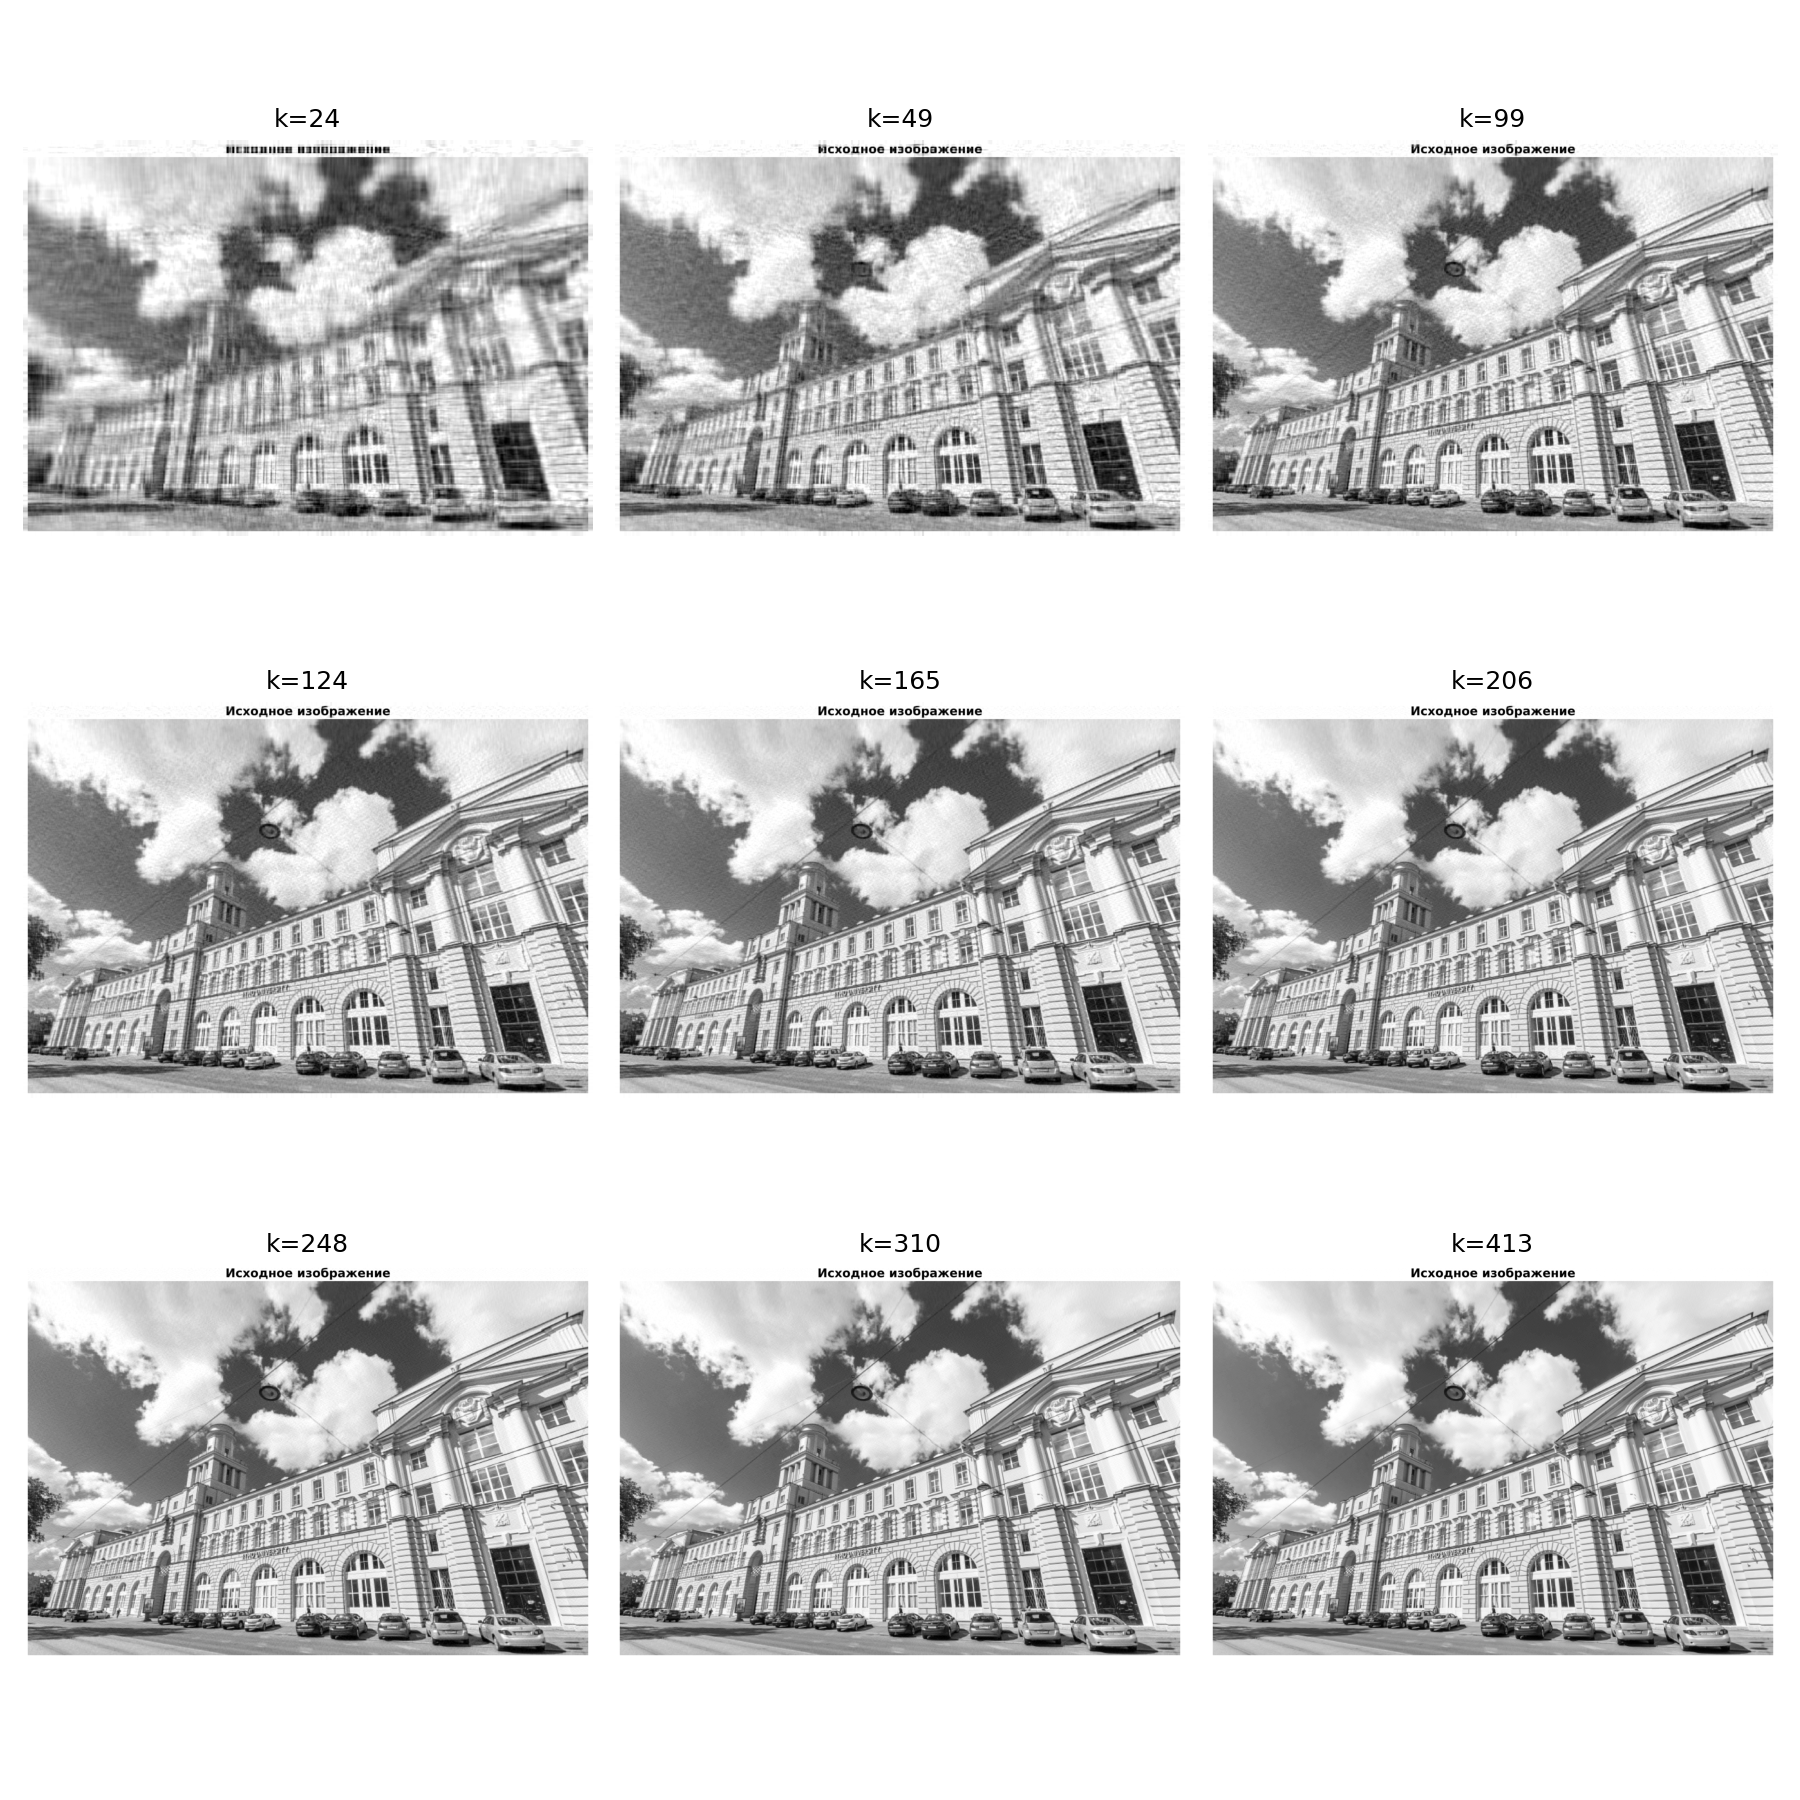
\includegraphics[width=0.95\linewidth]{images/task1/svd_grid.png}
  \caption{Реконструкции при различных \(k\) (9 вариантов)}
  \label{fig:svd-grid}
\end{figure}

\begin{figure}[h!]
  \centering
  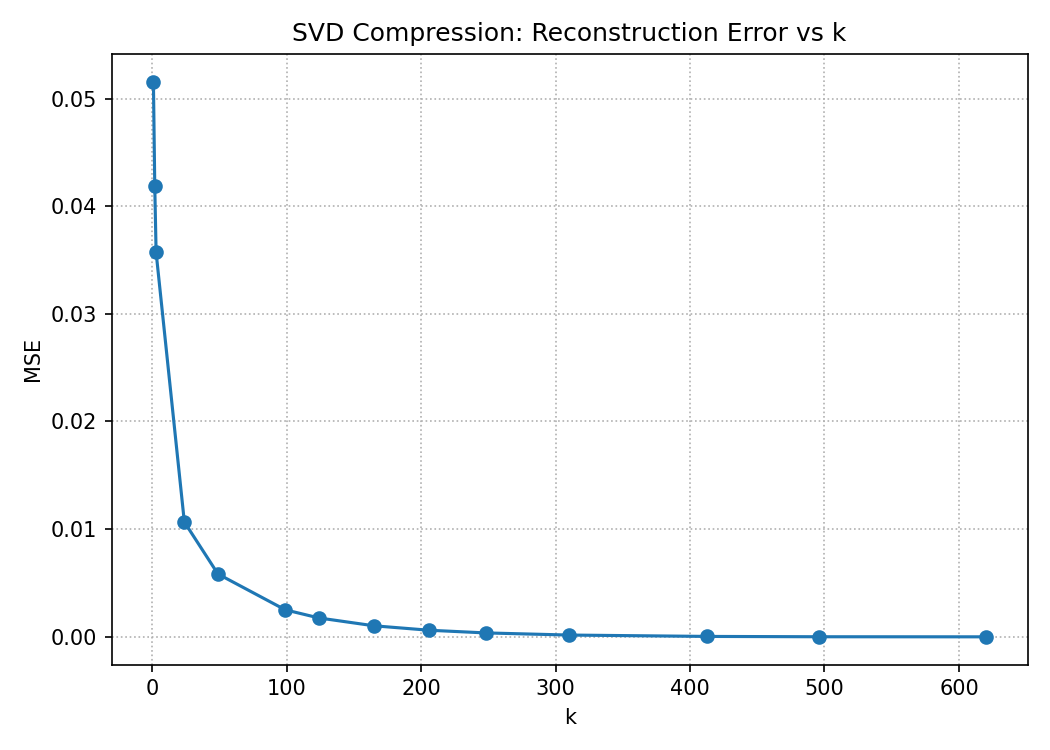
\includegraphics[width=0.48\linewidth]{images/task1/svd_mse_vs_k.png}\hfill
  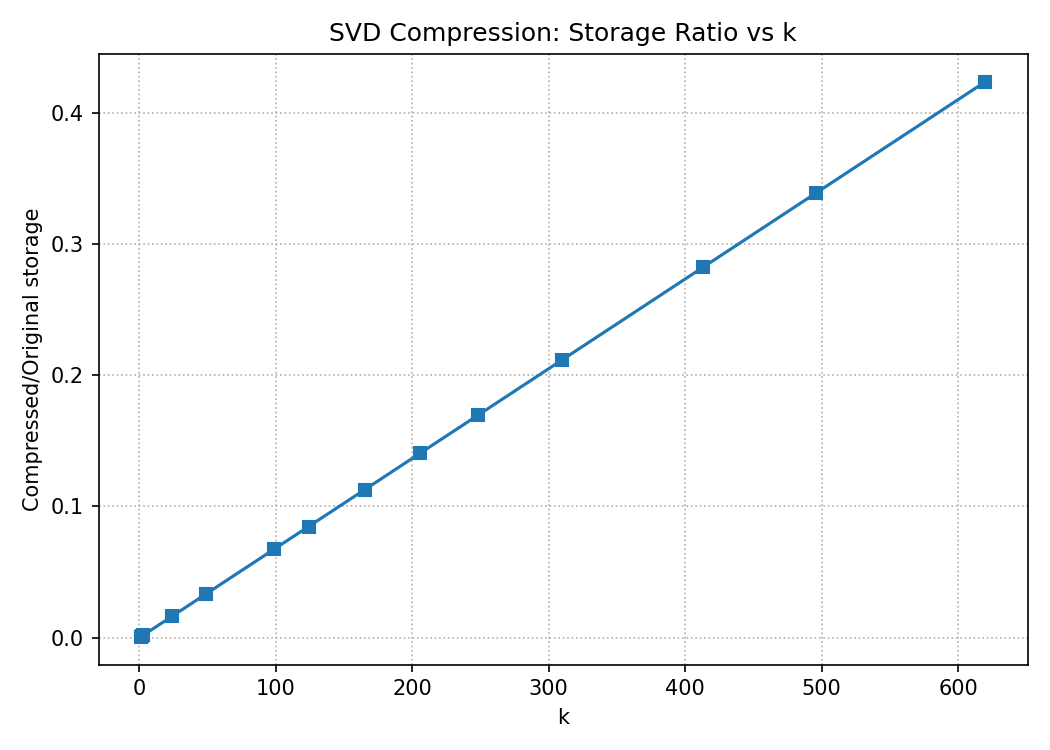
\includegraphics[width=0.48\linewidth]{images/task1/svd_storage_ratio_vs_k.png}
  \caption{Зависимость ошибки (MSE) и относительного объёма хранения от \(k\)}
  \label{fig:svd-metrics}
\end{figure}

\subsection*{Анализ результатов}
\begin{itemize}
  \item При малых \(k\) (единицы) картинка сильно теряет детали и становится расплывчатой; она уже распознаваема, но качество невысокое.
  \item При средних \(k\) видны основные контуры и крупные детали; качество приемлемое при заметном снижении объёма хранения.
  \item При больших \(k\) визуально близко к исходному, но выигрыш по памяти меньше.
\end{itemize}

Численно степень сжатия оценивалась как
\[ \text{ratio}(k) = \frac{m k + k + k n}{m n}, \]
где числитель — количество значений для хранения укороченного разложения \(U_k,\Sigma_k,V_k\). Для представленных значений \(k\) график на рисунке~\ref{fig:svd-metrics} показывает компромисс между качеством (MSE) и объёмом хранения.

\section*{Задание 2. Latent Semantic Analysis (LSA)}

Для набора текстовых документов был выполнен предобработчик: удаление пунктуации и цифр, приведение к нижнему регистру, токенизация, лемматизация (\texttt{pymorphy2}) и исключение стоп-слов (\texttt{nltk}). По очищенной коллекции построена терм-документная матрица (TF–IDF-подобное взвешивание), затем выполнено SVD-разложение.

Ниже приведены: спектр сингулярных чисел, а также визуализации двух тем — топ-5 слов в каждой теме и облака слов.

\begin{figure}[h!]
  \centering
  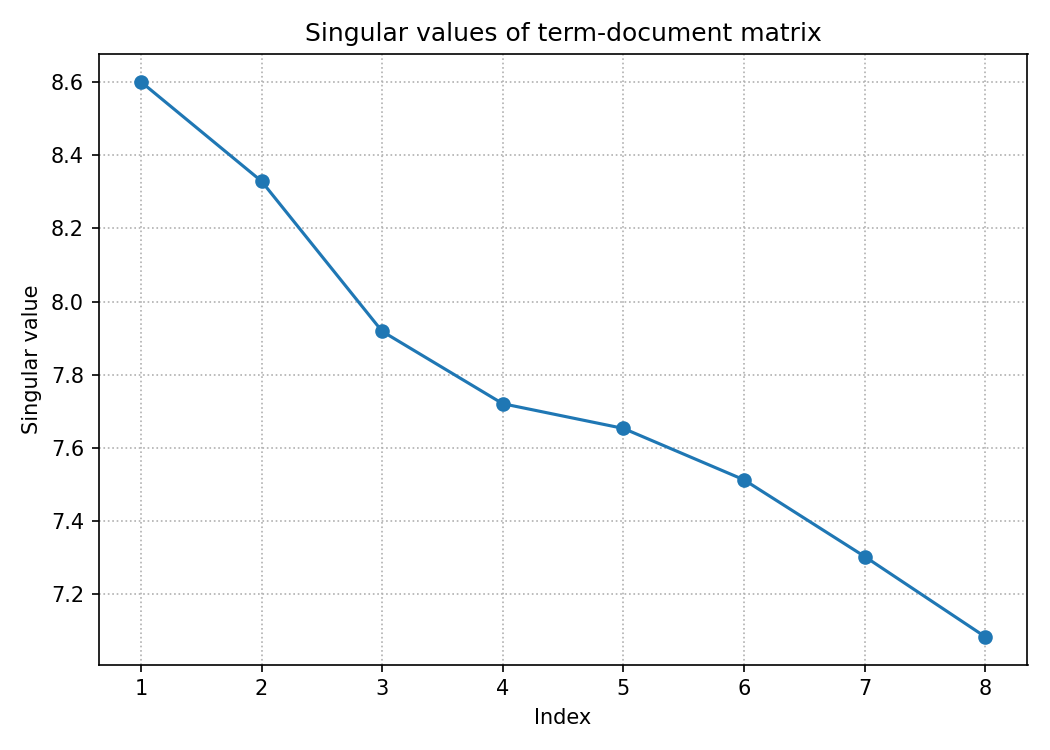
\includegraphics[width=0.6\linewidth]{images/task2/singular_values.png}
  \caption{Сингулярные числа терм-документной матрицы}
  \label{fig:lsa-svals}
\end{figure}

\begin{figure}[h!]
  \centering
  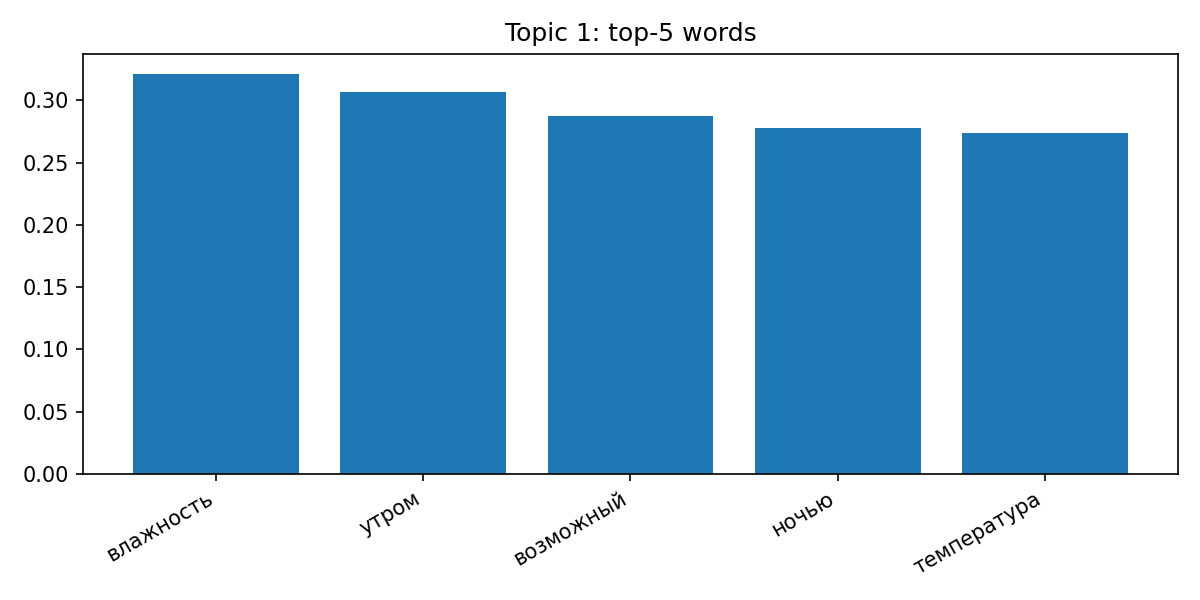
\includegraphics[width=0.48\linewidth]{images/task2/topic1_top_words.png}\hfill
  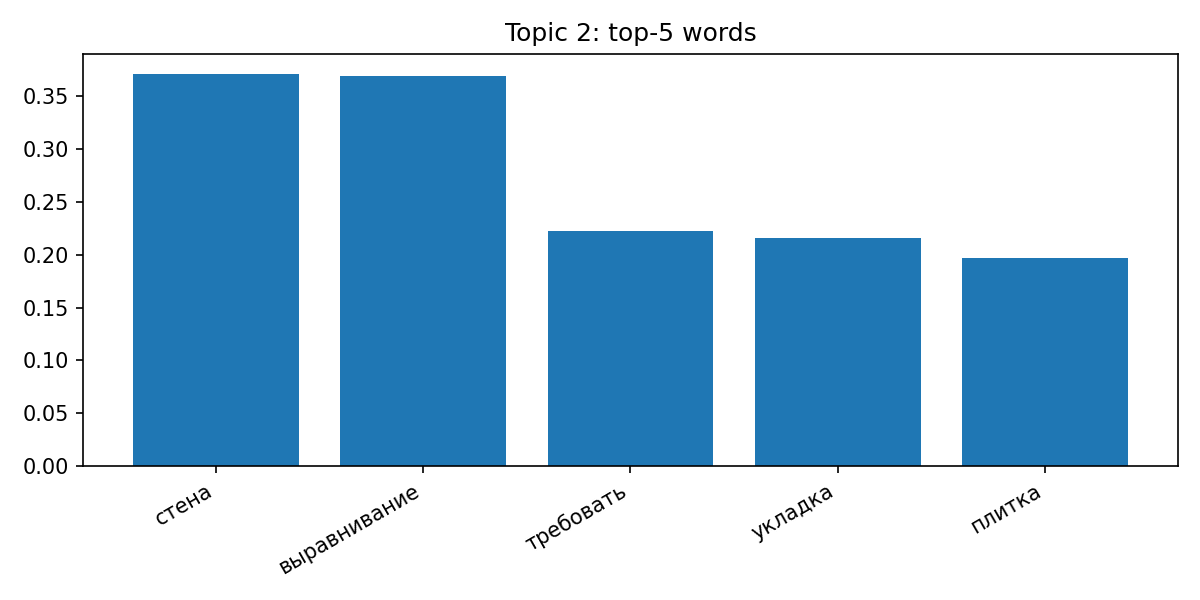
\includegraphics[width=0.48\linewidth]{images/task2/topic2_top_words.png}
  \caption{Топ-5 слов по абсолютному вкладу в двух ведущих темах}
  \label{fig:lsa-topwords}
\end{figure}

\begin{figure}[h!]
  \centering
  
\includegraphics[width=0.48\linewidth]{images/task2/topic1_wordcloud.png}\hfill
  
\includegraphics[width=0.48\linewidth]{images/task2/topic2_wordcloud.png}
  \caption{Облака слов для двух тем}
  \label{fig:lsa-wordcloud}
\end{figure}

\subsection*{Краткий анализ}
Первая и вторая сингулярные компоненты отражают две главные латентные темы в коллекции. Слова с наибольшими по модулю весами в соответствующих векторах \(U\) формируют смысловое ядро тем; компоненты вектора \(V\) позволяют определить документы, максимально связанные с каждой темой. После получения входного файла будут добавлены конкретные формулировки тем и номера документов, наиболее им соответствующие.

Для использованного примера (см. рис.~\ref{fig:lsa-topwords},~\ref{fig:lsa-wordcloud}) темы интерпретируются так: Тема 1 — спортивная (\emph{команд, игр, баскетбол, атак, матч}); сильнее всего связаны документы Doc~8, Doc~3, Doc~4. Тема 2 — технологическая/научная (\emph{нов, улучш, журнал, результат, научн}); сильнее всего связаны документы Doc~7 и Doc~1.

\section*{Выводы по проделанной работе}
\begin{itemize}
  \item По задаче SVD-сжатия: при малых \(k\) изображение заметно теряет детали; при средних \(k\) качество уже приемлемое при разумном уменьшении объёма хранения; при больших \(k\) картинка близка к исходной, но выигрыш по памяти снижается. Характерная зависимость MSE и доли хранения от \(k\) подтверждает ожидаемый компромисс «качество–сжатие».
  \item По задаче LSA: базовая предобработка и SVD позволяют выделить в корпусе несколько устойчивых тем. Для примера получили спортивную и технологическую/научную темы; соответствующие документы выделяются по весам правых сингулярных векторов. Убывание сингулярных чисел указывает на наличие низкоранговой структуры.
\end{itemize}

